\section{Kinds}
\topics{Kinds and data type promotion}

\emph{Kinds} are the ``types of types''. While types describe the sort of values that an expression may evaluate to and prevent us from writing \emph{e.g.} functions that break at runtime, kinds are useful to prevent us from doing ``wrong'' things with types themselves. For example, we know that a type constructor such as \haskellIn{Maybe} is parametrised over a type and must therefore be applied to one type as argument before \haskellIn{Maybe} yields a type itself. Kinds formalise this idea and allow us to say that \emph{e.g.} \haskellIn{Maybe} is of kind \haskellIn{* -> *}. The kind \haskellIn{*} represents all types and the kind \haskellIn{* -> *} represents all type constructors which expect a single type as argument before yielding a type themselves, such as \haskellIn{Maybe}. Therefore, \emph{e.g.} \haskellIn{Maybe Bool} is of kind \haskellIn{*}.

The skeleton code for these exercises can be obtained as usual with the following command:
\begin{minted}{bash}
$ git clone https://github.com/fpclass/lab-kinds
\end{minted}
Note that there are no tests for this lab and all exercises can be completed in the REPL which can be opened as usual with \texttt{\small stack repl}. There are some commands that are supported by the REPL which you may find useful for this set of exercises and for the exercises on \emph{Type-level programming}:
\begin{center}
	\begin{tabular}{|l|l|}
		\hline 
		\texttt{\small :k TYPE}   & Infers the kind of \texttt{\small TYPE}. \\ 
		\hline 
		\texttt{\small :kind!~TYPE}  & Reduces \texttt{\small TYPE} to a normal form. \\ 
		\hline 
	\end{tabular} 
\end{center}

\taskLine

\task{Just like you can ask the Haskell compiler to infer the types of expressions for you, you can also ask it to infer the kinds of types for you. Try running the following commands in the REPL to validate that what we described above is correct:}
\begin{itemize}
	\item \texttt{\small :k Maybe} 
	\item \texttt{\small :k Maybe Bool} 
	\item \texttt{\small :k Maybe Int} 
	\item \texttt{\small :k Maybe (Maybe Bool)} 
	\item \texttt{\small :k []}
	\item \texttt{\small :k [Bool]}  
\end{itemize}

\pagebreak

\task{What is the kind of the \haskellIn{Compose} type from the exercises about functors?}
\begin{minted}{haskell}
data Compose f g a = Compose (f (g a))
\end{minted}

\taskLine

\task{GHC provides type-level booleans out-of-the-box for us. Ordinarily, we can think of the \haskellIn{Bool} type as follows:}

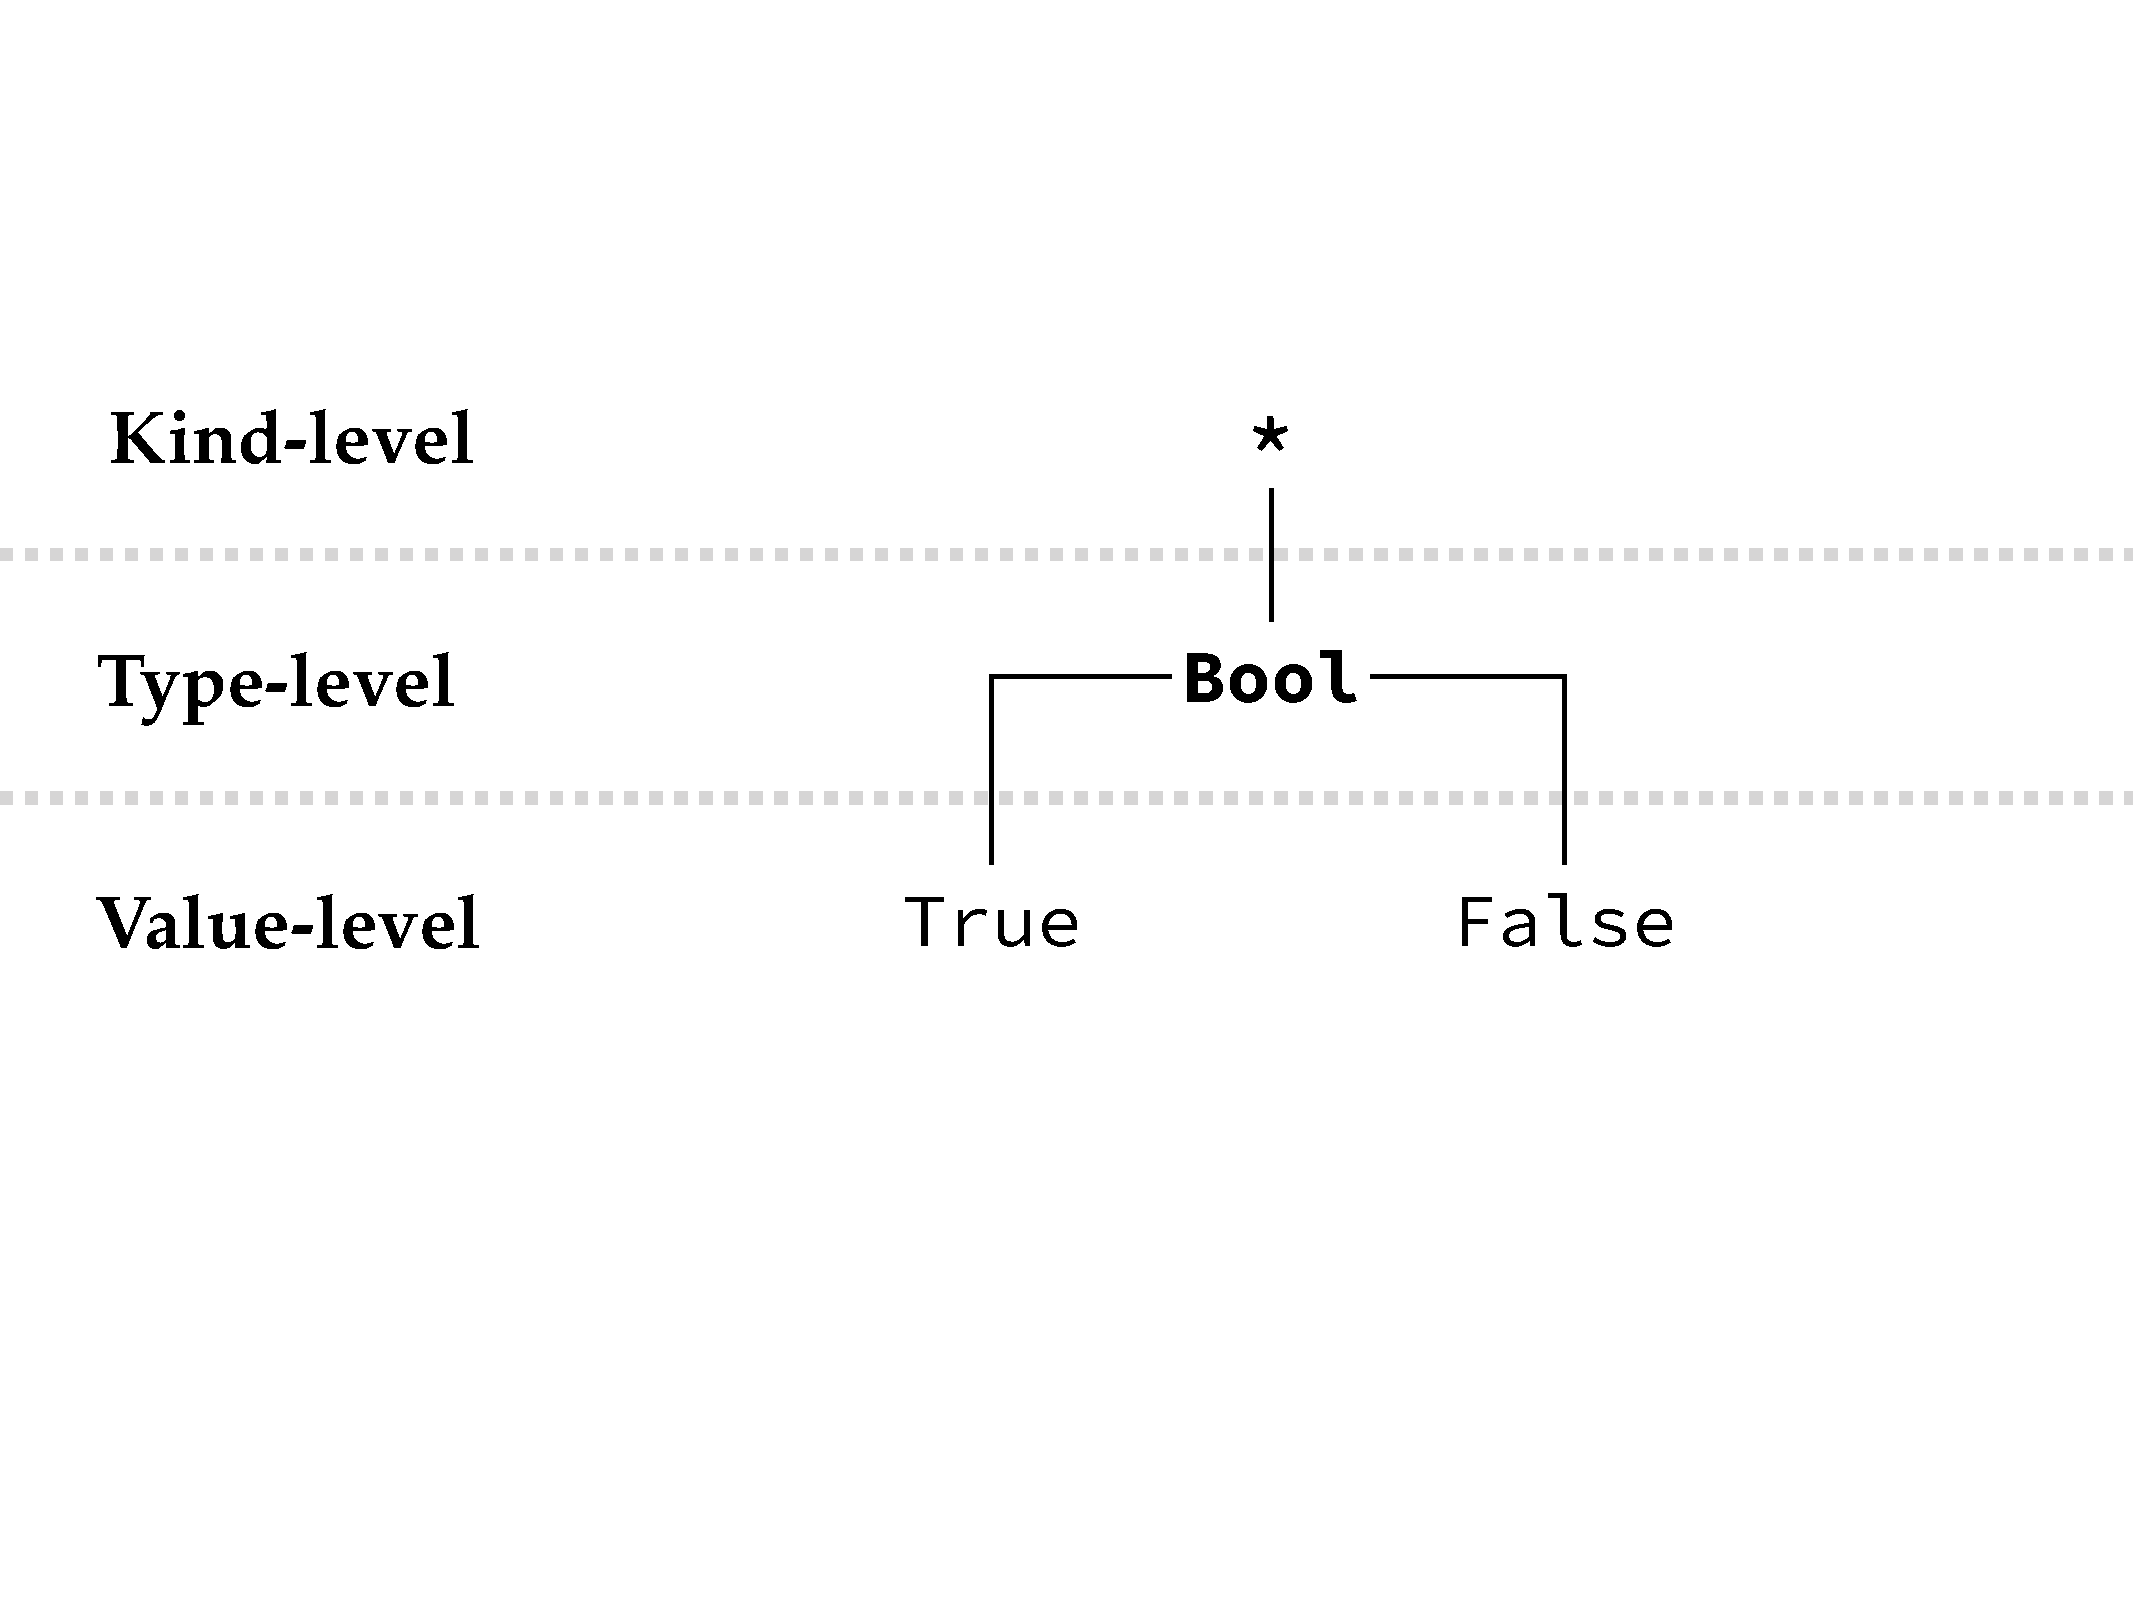
\includegraphics[clip, trim=0cm 10cm 0cm 6cm, width=1.00\textwidth]{labs/bool.pdf}

That is, \haskellIn{Bool} is a type and there are two values of this type: \haskellIn{True} and \haskellIn{False}. As an ordinary type, it is of kind \haskellIn{*} (read as \emph{type}). With \texttt{\small -XDataKinds} (\emph{i.e.} type promotion) enabled, the \texttt{\small Bool} type is automatically promoted to its own kind and its data constructors, \haskellIn{True} and \haskellIn{False}, are automatically promoted to types of that kind, all \emph{in addition to the above}. We can visualise this as:

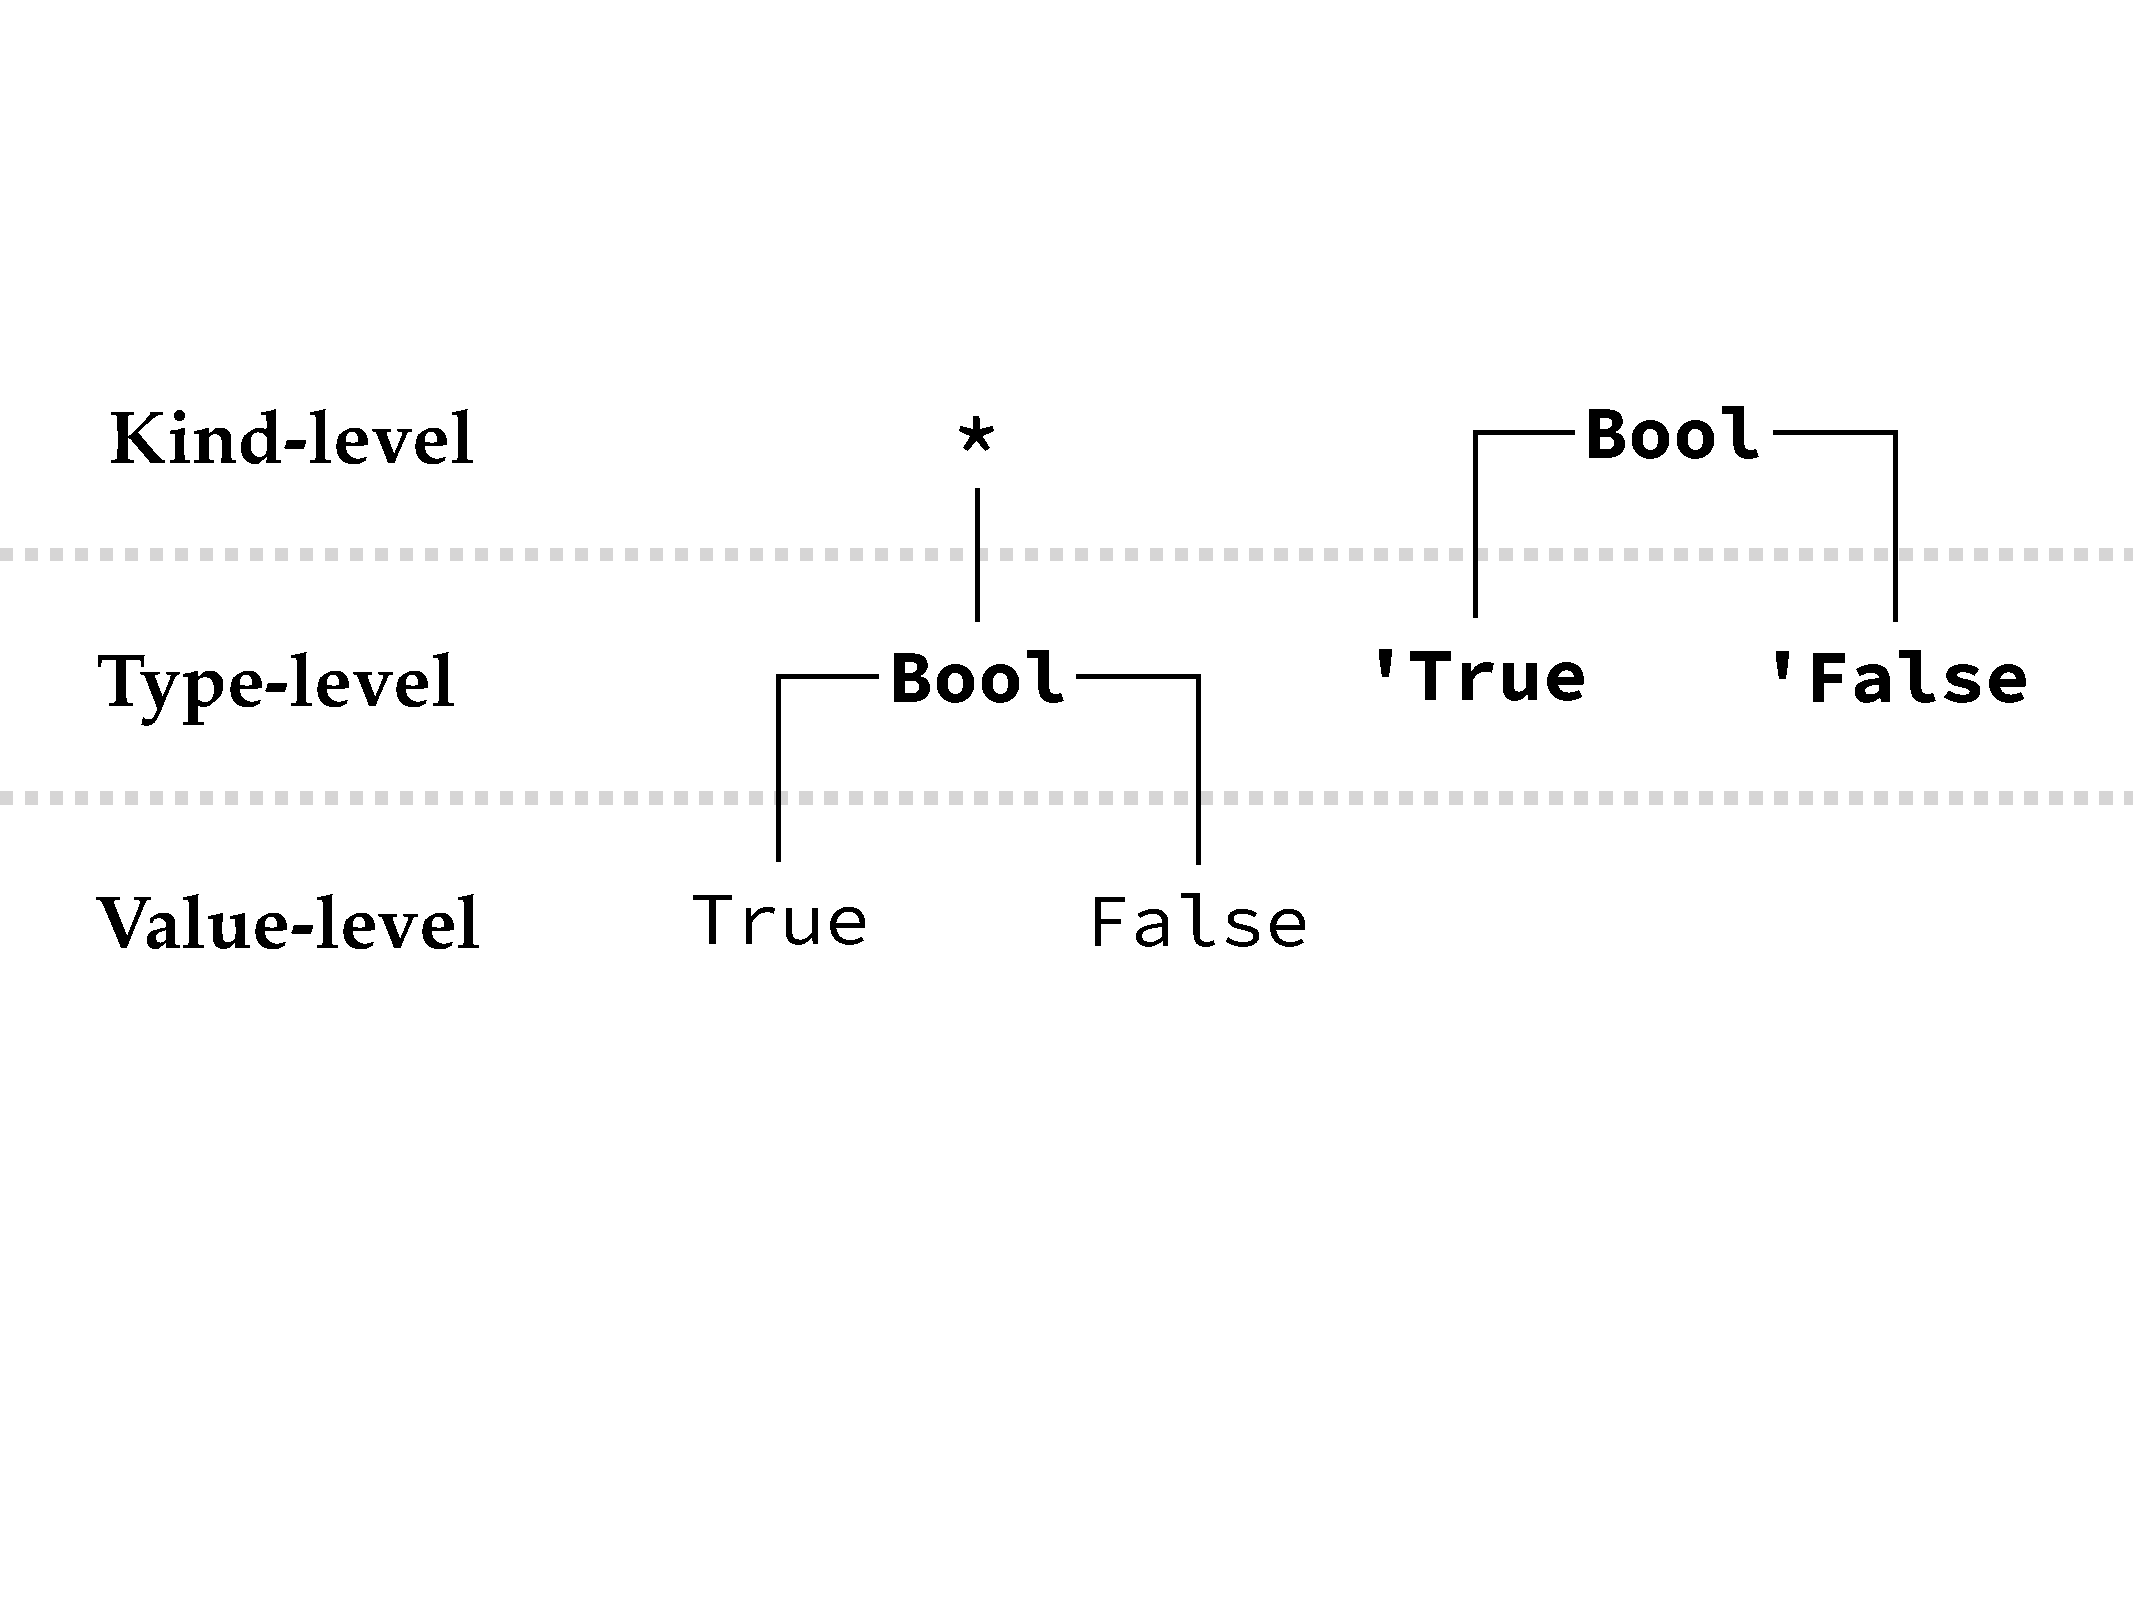
\includegraphics[clip, trim=0cm 10cm 0cm 6cm, width=1.00\textwidth]{labs/bool-promoted.pdf}

In addition to the \haskellIn{Bool} type with its \haskellIn{True} and \haskellIn{False} constructors, we now have a kind that is also named \haskellIn{Bool}. There are two types of kind \haskellIn{Bool}: \haskellIn{'True} and \haskellIn{'False}. Run the following commands in the REPL to validate what we have described:
\begin{itemize}
	\item \texttt{\small :k Bool} 
	\item \texttt{\small :t True} 
	\item \texttt{\small :k 'True} 
	\item \texttt{\small :k True} 
\end{itemize}
Note that the last two commands are the same. Because types and values are different namespaces, we can often just write \haskellIn{True} instead of \haskellIn{'True} to refer to the type named \haskellIn{True}. However, to avoid ambiguity it is always good practice to explicitly include the \texttt{'}.

\taskLine

\task{GHC also provides type-level lists out-of-the-box for us when \texttt{\small -XDataKinds} is enabled. Try the following in the REPL:}
\begin{itemize}
	\item \texttt{\small :k []}
	\item \texttt{\small :t (:)}
	\item \texttt{\small :t []}
	\item \texttt{\small :k '[]}
	\item \texttt{\small :k (:)}
	\item \texttt{\small :k Int :~'[]}
\end{itemize}